% ============================================================
%  Phương pháp tuyến tính cho giảm chiều dữ liệu
% ============================================================

% ------ Frame 1: Giả định tuyến tính ------
\begin{frame}{Giảm chiều tuyến tính: giả định và trực giác hình học}
	\setlength{\intextsep}{0.2em}
	\setlength{\columnsep}{0.8em}
	\begin{wrapfigure}{r}{0.42\textwidth}
		\centering
		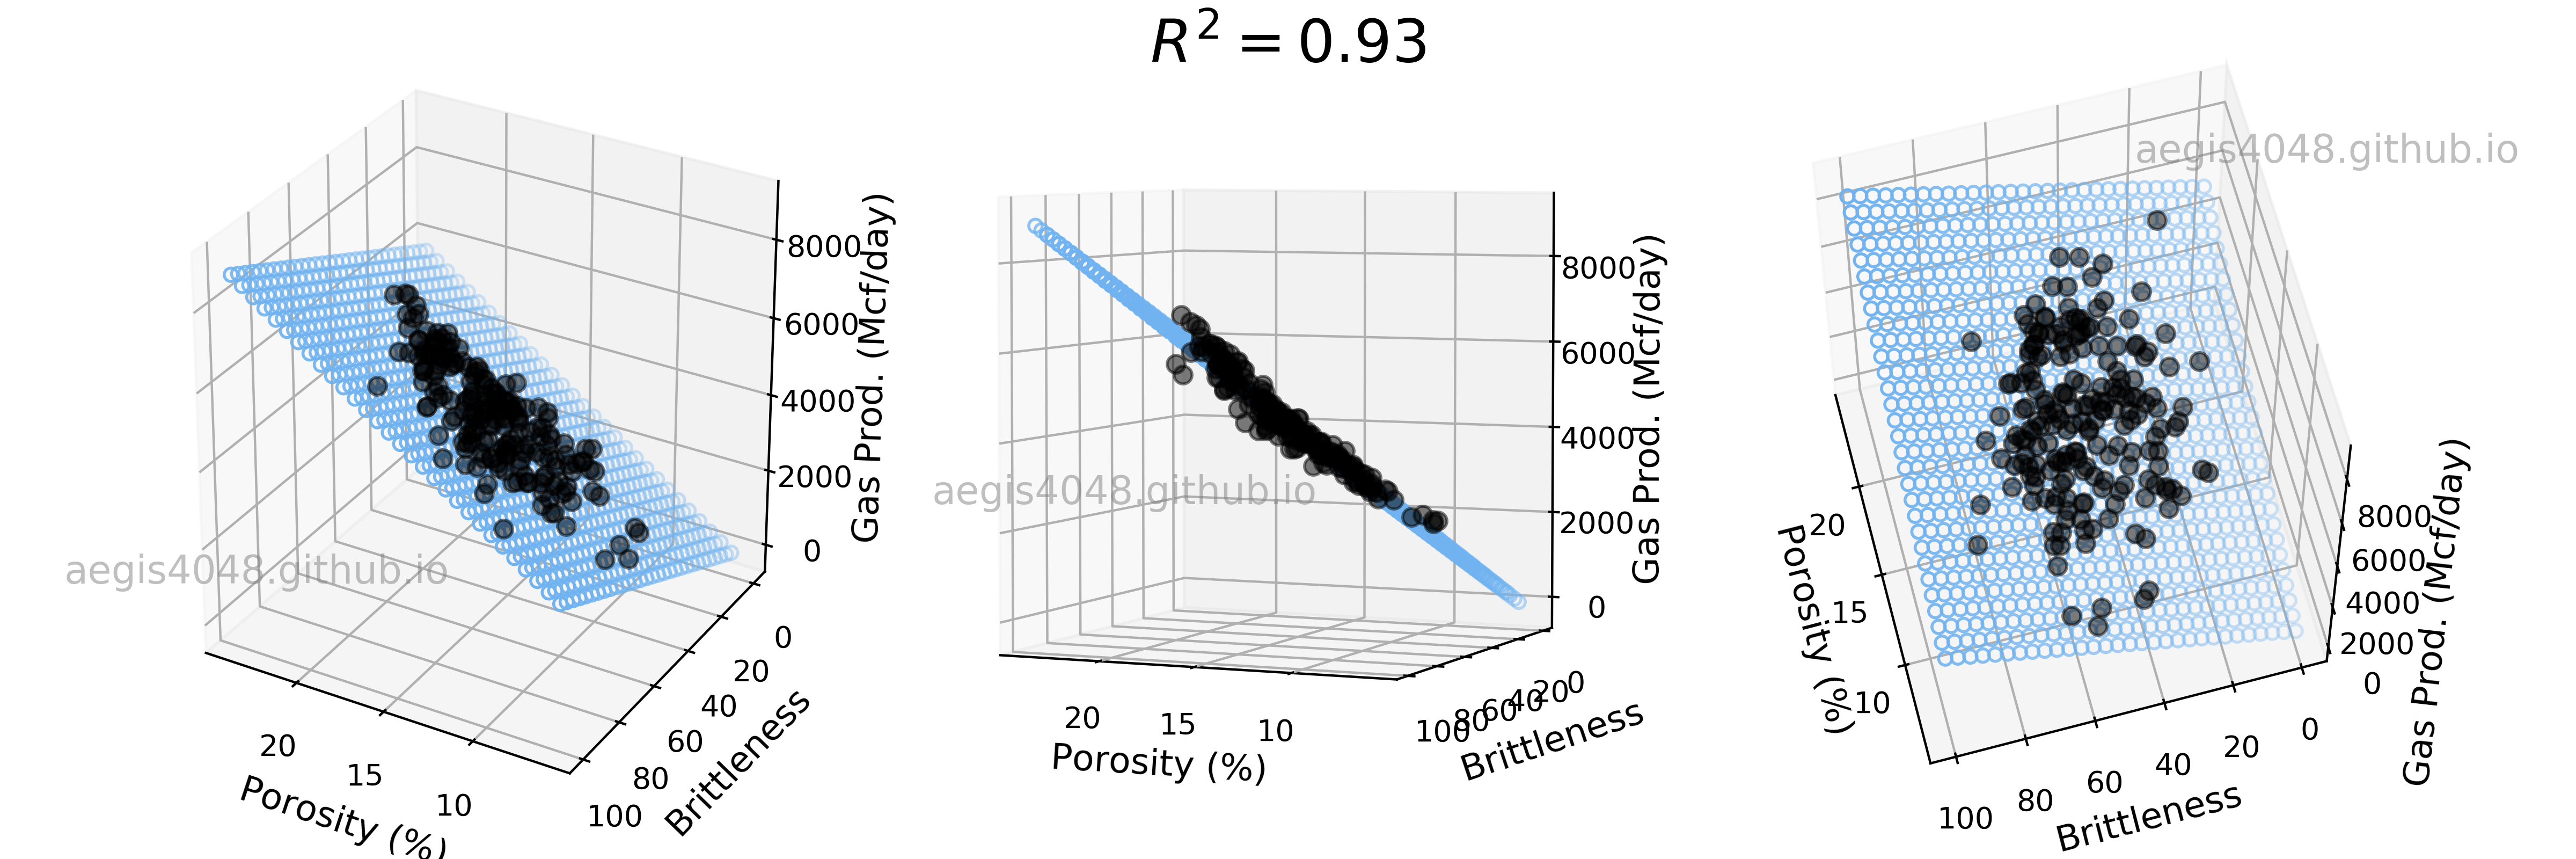
\includegraphics[width=0.98\linewidth]{img/Chapter2/linearity.png}
		\\
		{\scriptsize Minh họa dữ liệu gần không gian con tuyến tính.}
	\end{wrapfigure}

	\textbf{Giả định tuyến tính (linearity assumption)}
	\vspace{0.2em}

	\begin{itemize}
		\item Dữ liệu trong không gian cao chiều thường nằm gần một \textbf{không gian con tuyến tính} thấp chiều.
		\item Mỗi điểm $\mathbf{x}\in\mathbb{R}^P$ xấp xỉ: $\mathbf{x} \approx \sum_{i=1}^{K} z_i\mathbf{w}_i + \boldsymbol{\epsilon}$, với $K \ll P$.
		\item Thông tin quan trọng tập trung ở vài hướng biến thiên lớn; phần còn lại thường là nhiễu hoặc dư thừa.
	\end{itemize}

	\vspace{0.2em}
	\begin{block}{Tại sao bắt đầu với giả định tuyến tính?}
		Mô hình đơn giản nhất (Occam's Razor) $\;\Rightarrow\;$ dẫn đến bài toán tối ưu có \textbf{lời giải giải tích} qua phân tích ma trận (Eigendecomposition, SVD).
	\end{block}

	\hfill{\scriptsize Theo \cite{duchesnay2021statsml,lequocnghi2020}}
\end{frame}

% ------ Frame 2: Ứng dụng thực tế của giả định tuyến tính ------
\begin{frame}{Giả định tuyến tính trong thực tế}
	\small
	\begin{columns}[T]
		\column{0.55\textwidth}
		\begin{itemize}
			\item \textbf{Xử lý ảnh khuôn mặt (Eigenfaces):} \\ Biểu diễn xấp xỉ tốt trong không gian con tuyến tính của không gian pixel — giảm từ hàng nghìn chiều xuống vài chục thành phần chính mà vẫn nhận dạng được.
			\item \textbf{Kinh tế-xã hội:} \\ Tương quan tuyến tính mạnh giữa các biến $\Rightarrow$ \\ $>90\%$ phương sai bảo toàn với rất ít thành phần chính.
			\item \textbf{Sinh học tính toán:} \\ Dữ liệu biểu hiện gen (hàng nghìn chiều) thường nằm xung quanh vài con đường sinh học tuyến tính.
		\end{itemize}

		\column{0.42\textwidth}
		\centering
		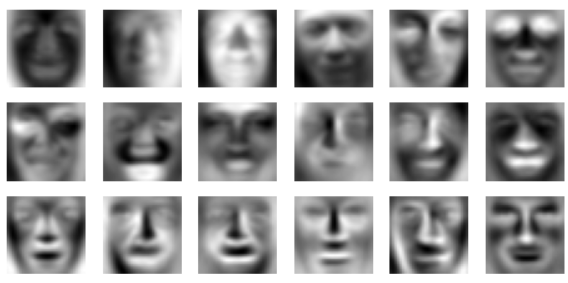
\includegraphics[width=0.95\linewidth]{img/Chapter2/PCA-face.png}
		\\
		{\scriptsize Đặc trưng khuôn mặt được bảo toàn trong không gian con tuyến tính sau giảm chiều.}
	\end{columns}
\end{frame}

% ------ Frame 3: Phát biểu bài toán ------
\begin{frame}{Phát biểu bài toán giảm chiều tuyến tính}
	Với dữ liệu $\mathbf{X}\in\mathbb{R}^{N\times P}$, cần tìm không gian con $K$ chiều ($K<P$) giữ lại thông tin quan trọng.

	\vspace{0.3em}
	\begin{enumerate}
		\item \textbf{Biến cần tìm:} ma trận cơ sở $\mathbf{V}\in\mathbb{R}^{P\times K}$ và biểu diễn thấp chiều $\mathbf{U}\in\mathbb{R}^{N\times K}$.
		\item \textbf{Phép chiếu:}
		\[
			\mathbf{U}=\mathbf{X}\mathbf{V}
		\]
		\item \textbf{Phép tái tạo:}
		\[
			\hat{\mathbf{X}}=\mathbf{U}\mathbf{V}^T,\qquad \mathbf{X}\approx \hat{\mathbf{X}}
		\]
		\item \textbf{Hàm mục tiêu phổ biến (PCA):}
		\[
			\min_{\mathbf{V}}\left\|\mathbf{X}-\mathbf{X}\mathbf{V}\mathbf{V}^T\right\|_F^2
		\]
	\end{enumerate}

\end{frame}

% ------ Frame 4: Minh họa phân rã ma trận ------
\begin{frame}{Phân rã ma trận trong giảm chiều tuyến tính}
	\begin{center}
		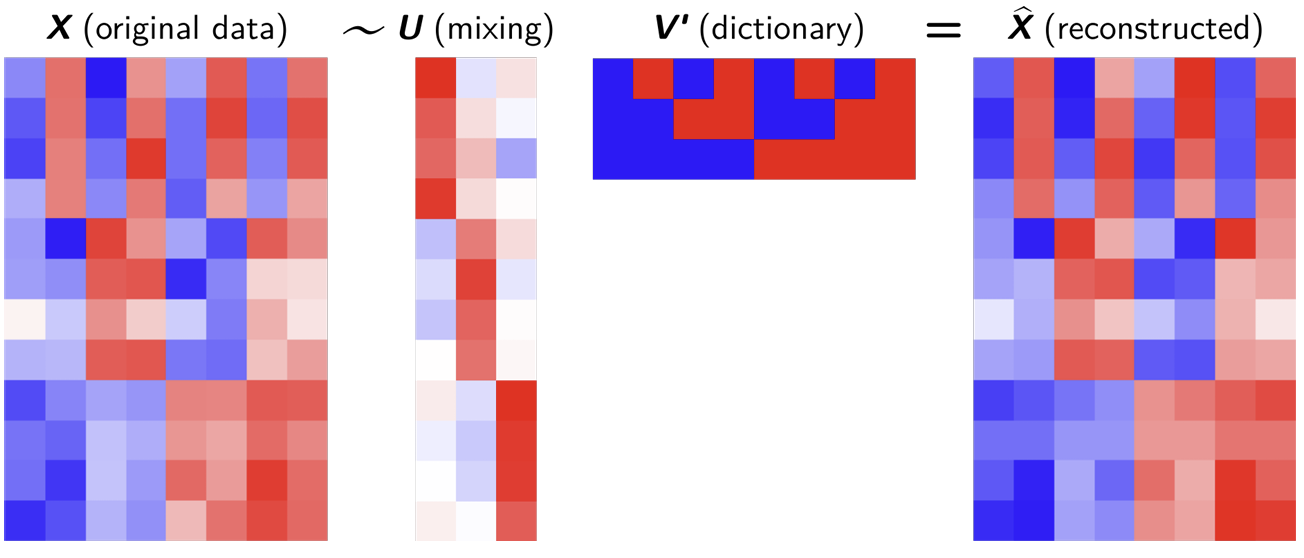
\includegraphics[width=0.82\linewidth]{img/Chapter2/matrix-factorisation.png}
		\\[0.4em]
		{\small Phân rã $\mathbf{X} \approx \mathbf{U}\mathbf{V}^T$: ma trận hệ số $\mathbf{U}$ ($N\times K$) và ma trận cơ sở $\mathbf{V}$ ($P\times K$).}
	\end{center}
\end{frame}

% ------ Frame 5: PCA định nghĩa ------
\begin{frame}{PCA: định nghĩa và mục tiêu}
	\small
	\begin{itemize}
		\item PCA biến đổi dữ liệu từ không gian $P$ chiều sang không gian $K$ chiều ($K<P$) sao cho các biến mới \textbf{không tương quan tuyến tính}.
		\item Tìm ma trận chiếu trực giao $\mathbf{V}\in\mathbb{R}^{P\times K}$ để \textbf{tối đa hóa phương sai} theo các hướng chiếu.
		\item Mục tiêu: bảo toàn tối đa thông tin quan trọng trong số chiều nhỏ hơn.
	\end{itemize}

	\vspace{0.3em}
	\[
		\mathbf{Z}=\mathbf{X}_c\mathbf{V}_K,\qquad
		\mathbf{X}_c=\mathbf{X}-\mathbf{1}\bar{\mathbf{x}}^T
	\]

	\begin{block}{Ý nghĩa hình học}
		Các trục tọa độ mới là các hướng biến thiên mạnh nhất của đám mây dữ liệu — trục chính của khối ellipsoid bao quanh dữ liệu.
	\end{block}
\end{frame}

% ------ Frame 6: Trực giác hình học PCA ------
\begin{frame}{Trực giác hình học của PCA}
	\setlength{\columnsep}{0.8em}
	\begin{columns}[T]
		\column{0.5\textwidth}
		\centering
		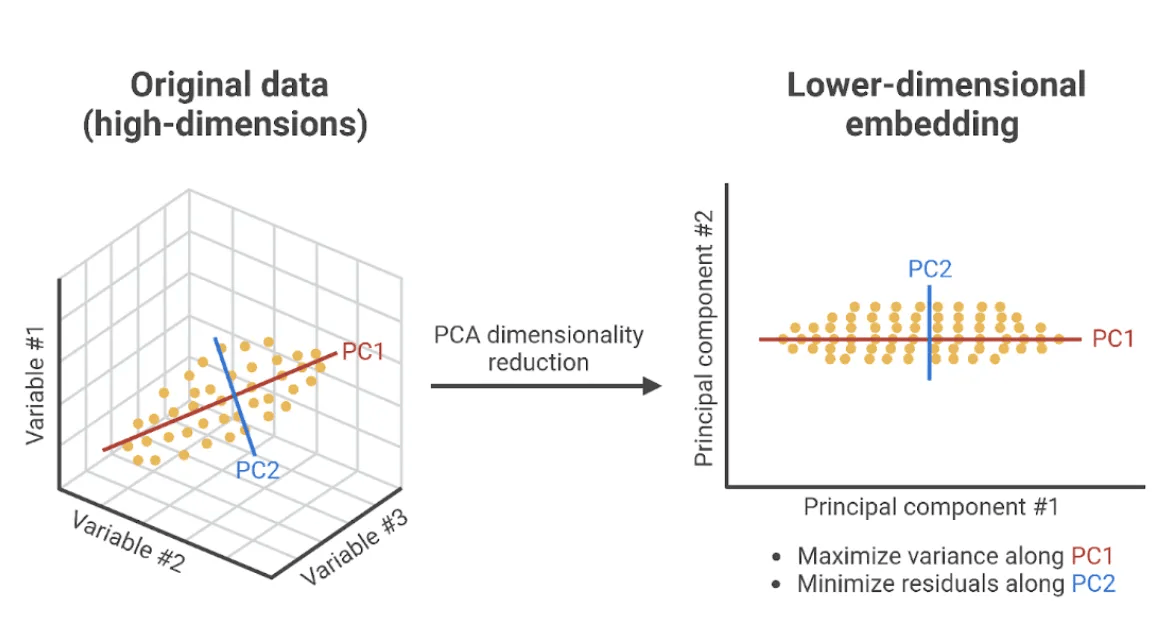
\includegraphics[width=0.95\linewidth]{img/Chapter2/PCA-example.png}
		\\
		{\scriptsize Chiếu dữ liệu lên không gian con $K$ chiều qua $\mathbf{V}$.}

		\column{0.5\textwidth}
		\centering
		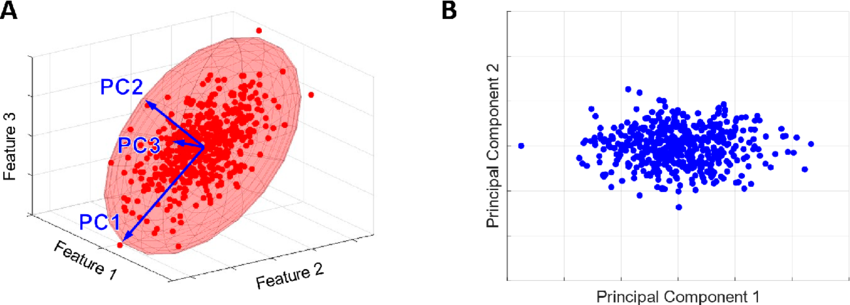
\includegraphics[width=0.95\linewidth]{img/Chapter2/PCA-geo-example.png}
		\\
		{\scriptsize Ellipsoid dữ liệu và các trục chính (thành phần chính).}
	\end{columns}

	\vspace{0.3em}
	\small
	\begin{itemize}
		\item Giữ $K$ trục ellipsoid \textbf{dài nhất} $\Rightarrow$ giữ phương sai lớn nhất.
		\item Loại bỏ các trục phương sai thấp, thường gắn với nhiễu/dư thừa.
	\end{itemize}
\end{frame}

% ------ Frame 7: PCA Eigendecomposition bước 1-2 ------
\begin{frame}{PCA truyền thống (Eigendecomposition)}
	\small
	\textbf{Bước 1: Tiền xử lý dữ liệu}
	\begin{itemize}
		\item Trung tâm hóa (centering):
	\end{itemize}
	\[
		\mathbf{X}_c = \mathbf{X} - \mathbf{1}\bar{\mathbf{x}}^T
	\]
	\begin{itemize}
		\item Nếu các biến khác thang đo: \textbf{chuẩn hóa} theo độ lệch chuẩn để tránh biến phương sai lớn chi phối kết quả.
	\end{itemize}

	\vspace{0.3em}
	\textbf{Bước 2: Ma trận hiệp phương sai}
	\[
		\mathbf{S}_{XX}=\frac{1}{N-1}\mathbf{X}_c^T\mathbf{X}_c \;\in\mathbb{R}^{P\times P}
	\]
	\begin{itemize}
		\item Đánh giá mức độ biến thiên và tương quan giữa tất cả các cặp đặc trưng.
	\end{itemize}
\end{frame}

% ------ Frame 8: PCA Eigendecomposition bước 3-4 ------
\begin{frame}{PCA truyền thống (Eigendecomposition)}
	\small
	\textbf{Bước 3: Tìm hướng chiếu tối ưu}
	\[
		\mathbf{v}=\arg\max_{\|\mathbf{v}\|=1}\mathbf{v}^T\mathbf{S}_{XX}\mathbf{v}
		\;\xrightarrow{\text{Lagrange}}\;
		\mathbf{S}_{XX}\mathbf{v}=\lambda\mathbf{v}
	\]
	\begin{itemize}
		\item $\mathbf{v}$ là \textbf{eigenvector}, $\lambda$ là \textbf{eigenvalue} (= phương sai theo hướng đó).
		\item Chọn $K$ eigenvalue lớn nhất: $\lambda_1\ge\lambda_2\ge\dots\ge\lambda_K$.
		\item Tạo ma trận chiếu $\mathbf{V}_K\in\mathbb{R}^{P\times K}$ từ các eigenvector tương ứng.
	\end{itemize}

	\vspace{0.2em}
	\textbf{Bước 4: Chiếu dữ liệu sang không gian mới}
	\[
		\mathbf{Z}=\mathbf{X}_c\mathbf{V}_K,\qquad \mathbf{Z}\in\mathbb{R}^{N\times K}
	\]
	\begin{itemize}
		\item $\mathbf{Z}$ có các đặc trưng \textbf{không tương quan tuyến tính} và giữ phần lớn thông tin quan trọng.
	\end{itemize}
\end{frame}

% ------ Frame 8.5: Ví dụ số PCA 2D -> 1D ------
\begin{frame}{Ví dụ số cụ thể: PCA từ 2D xuống 1D}
	\scriptsize
	\setlength{\abovedisplayskip}{0.2em}
	\setlength{\belowdisplayskip}{0.2em}
	\setlength{\abovedisplayshortskip}{0.15em}
	\setlength{\belowdisplayshortskip}{0.15em}
	\setlength{\columnsep}{0.6em}
	Cho 4 điểm dữ liệu trong $\mathbb{R}^2$:
	\[
		(2,1),\ (3,2),\ (4,3),\ (5,4)
	\]
	\begin{columns}[T]
		\column{0.51\textwidth}
		\textbf{Bước 1: Trung tâm hóa}
		\[
			\bar{\mathbf{x}}=(3.5,\,2.5)
		\]
		\[
			\mathbf{X}_c=
			\begin{bmatrix}
				-1.5 & -1.5\\
				-0.5 & -0.5\\
				\phantom{-}0.5 & \phantom{-}0.5\\
				\phantom{-}1.5 & \phantom{-}1.5
			\end{bmatrix}
		\]

		\textbf{Bước 2: Hiệp phương sai}
		\[
			\mathbf{S}_{XX}=\frac{1}{3}\mathbf{X}_c^T\mathbf{X}_c
			=\begin{bmatrix}5/3 & 5/3\\ 5/3 & 5/3\end{bmatrix}
		\]

		\column{0.47\textwidth}
		\textbf{Bước 3: Thành phần chính thứ nhất}
		\[
			\lambda_1=\frac{10}{3},\;\lambda_2=0,
			\quad
			\mathbf{v}_1=\frac{1}{\sqrt{2}}\begin{bmatrix}1\\1\end{bmatrix}
		\]

		\textbf{Bước 4: Chiếu 2D $\to$ 1D}
		\[
			\mathbf{z}=\mathbf{X}_c\mathbf{v}_1
			=\begin{bmatrix}
				-2.121\\
				-0.707\\
				\phantom{-}0.707\\
				\phantom{-}2.121
			\end{bmatrix}
		\]
		\[
			\hat{\mathbf{x}}_i=\bar{\mathbf{x}}+z_i\mathbf{v}_1
		\]

	\end{columns}
	\begin{block}{Kết quả}
		Các điểm được chiếu lên cùng một đường thẳng (đường chéo $y=x$), nên chỉ với 1 chiều đã bảo toàn toàn bộ phương sai ($\mathrm{EVR}=100\%$).
	\end{block}
\end{frame}



% ------ Frame 9: Vấn đề PCA truyền thống ------
\begin{frame}{Vấn đề của PCA truyền thống}
	\small
	\begin{itemize}
		\item Xây dựng hiệp phương sai tường minh: thời gian $O(NP^2)$, bộ nhớ $O(P^2)$.
		\item Giải bài toán trị riêng ma trận vuông lớn: $O(P^3)$.
		\item Khi chỉ cần $K\ll P$, việc tính toàn bộ phổ trị riêng là \textbf{lãng phí tài nguyên}.
		\item Dữ liệu đa cộng tuyến/nhiễu khiến $\mathbf{S}_{XX}$ \textbf{kém điều kiện (ill-conditioned)}, gây mất ổn định số học.
	\end{itemize}

	\begin{block}{Hệ quả}
		Ưu tiên tính \textbf{SVD trực tiếp} trên $\mathbf{X}_c$ để đạt ổn định số học và hiệu quả tính toán cao hơn.
	\end{block}
\end{frame}

% ------ Frame 10: Mối quan hệ SVD và PCA ------
\begin{frame}{Mối quan hệ toán học giữa SVD và PCA}
	\footnotesize
	Phân rã SVD của dữ liệu trung tâm hóa:
	\[
		\mathbf{X}_c=\mathbf{U}\mathbf{D}\mathbf{V}^T
	\]
	Thay vào ma trận hiệp phương sai mẫu:
	\[
		\mathbf{S}_{XX}=\frac{1}{N-1}\mathbf{X}_c^T\mathbf{X}_c
		=\frac{1}{N-1}({\mathbf{U}\mathbf{D}\mathbf{V}^T})^T({\mathbf{U}\mathbf{D}\mathbf{V}^T})
		=\mathbf{V}\!\left(\frac{\mathbf{D}^2}{N-1}\right)\!\mathbf{V}^T
	\]
	\[
		\Rightarrow\quad\mathbf{S}_{XX}\mathbf{v}_k=\underbrace{\frac{d_k^2}{N-1}}_{\lambda_k}\mathbf{v}_k
	\]
		\begin{itemize}
			\item Các \textbf{right-singular vectors} $\mathbf{V}$ $\equiv$ các eigenvectors của $\mathbf{S}_{XX}$.
			\item $\lambda_k=\dfrac{d_k^2}{N-1}$ là eigenvalue tương ứng.
			\item Tọa độ chiếu: $\mathbf{C}=\mathbf{X}_c\mathbf{V}=\mathbf{U}\mathbf{D}$ (không cần $\mathbf{S}_{XX}$!).
		\end{itemize}
\end{frame}

% ------ Frame 11: Triển khai PCA qua SVD ------
\begin{frame}{Triển khai PCA qua SVD}
	\small
	\textbf{Bước 1: Chọn ma trận Gram nhỏ hơn}
	\[
		\mathbf{G}=
		\begin{cases}
			\mathbf{X}_c^T\mathbf{X}_c\in\mathbb{R}^{P\times P}, & N\ge P\\
			\mathbf{X}_c\mathbf{X}_c^T\in\mathbb{R}^{N\times N}, & N<P
		\end{cases}
	\]
	{\small \textit{(Ví dụ: gene expression $N=100, P=10^4$ $\Rightarrow$ giảm $\sim 10{.}000$ lần chi phí.)}}

	\textbf{Bước 2: Eigendecomposition trên $\mathbf{G}$}
	\[
		d_i=\sqrt{\lambda_i},\quad i=1,\dots,\mathrm{rank}(\mathbf{X}_c)
		\qquad\text{Chi phí}\sim\min\!\left(O(P^3),O(N^3)\right)
	\]

	\textbf{Bước 3: Truy hồi thành phần còn thiếu}
	\[
		\mathbf{v}_i=\frac{1}{d_i}\mathbf{X}_c^T\mathbf{u}_i
		\quad\text{hoặc}\quad
		\mathbf{u}_i=\frac{1}{d_i}\mathbf{X}_c\mathbf{v}_i
	\]

	\begin{block}{Kết luận}
		SVD là \textbf{tiêu chuẩn vàng} trong các thư viện hiện đại nhờ ổn định số học và tiết kiệm bộ nhớ.
	\end{block}
\end{frame}

\begin{frame}{Áp dụng SVD cho ví dụ 2D $\to$ 1D (1/2)}
	\scriptsize
	\setlength{\abovedisplayskip}{0.2em}
	\setlength{\belowdisplayskip}{0.2em}
	\setlength{\abovedisplayshortskip}{0.15em}
	\setlength{\belowdisplayshortskip}{0.15em}
	\setlength{\columnsep}{0.6em}
	Với cùng dữ liệu đã trung tâm hóa ($N=4,\,P=2\Rightarrow N\ge P$):
	\[
		\mathbf{X}_c=
		\begin{bmatrix}
			-1.5 & -1.5\\
			-0.5 & -0.5\\
			\phantom{-}0.5 & \phantom{-}0.5\\
			\phantom{-}1.5 & \phantom{-}1.5
		\end{bmatrix}
	\]
\textbf{Bước 1: Chọn Gram nhỏ hơn}
\[
	\mathbf{G}=\mathbf{X}_c^T\mathbf{X}_c=
	\begin{bmatrix}5 & 5\\ 5 & 5\end{bmatrix}
\]

\textbf{Bước 2: Eigendecomposition trên $\mathbf{G}$}
\[
	\lambda_1(\mathbf{G})=10,\;\lambda_2(\mathbf{G})=0
	\Rightarrow
	d_1=\sqrt{10},\;d_2=0
\]
\[
	\mathbf{v}_1=\frac{1}{\sqrt{2}}\begin{bmatrix}1\\1\end{bmatrix},\;
	\mathbf{v}_2=\frac{1}{\sqrt{2}}\begin{bmatrix}1\\-1\end{bmatrix}
\]
\end{frame}

\begin{frame}{Áp dụng SVD cho ví dụ 2D $\to$ 1D (2/2)}
	\scriptsize
	\setlength{\abovedisplayskip}{0.2em}
	\setlength{\belowdisplayskip}{0.2em}
	\setlength{\abovedisplayshortskip}{0.15em}
	\setlength{\belowdisplayshortskip}{0.15em}
	\setlength{\columnsep}{0.6em}
	\textbf{Bước 3: Truy hồi thành phần còn thiếu}
	\[
		\mathbf{u}_1=\frac{1}{d_1}\mathbf{X}_c\mathbf{v}_1
		=\frac{1}{\sqrt{20}}\begin{bmatrix}-3\\-1\\1\\3\end{bmatrix}
	\]
	\[
		\mathbf{X}_c=\mathbf{U}\mathbf{D}\mathbf{V}^T
	\]

	\textbf{Tọa độ 1D (giữ $K=1$)}
	\[
		\mathbf{z}=\mathbf{U}_1\mathbf{D}_1
		=\mathbf{X}_c\mathbf{v}_1
		=\begin{bmatrix}-2.121\\-0.707\\0.707\\2.121\end{bmatrix}
	\]
	\[
		\lambda_1=\frac{d_1^2}{N-1}=\frac{10}{3}
	\]
\end{frame}

% ------ Frame 12: Độ phức tạp tính toán ------
\begin{frame}{Độ phức tạp tính toán và so sánh hiệu năng}
	\footnotesize
	\renewcommand{\arraystretch}{1.35}
	\begin{tabular}{|p{2.8cm}|p{2.5cm}|p{2cm}|p{6cm}|}
		\hline
		\textbf{Phương pháp} & \textbf{Thời gian} & \textbf{Bộ nhớ} & \textbf{Nhận xét} \\
		\hline
		PCA truyền thống & $O(NP^2+P^3)$ & $O(P^2)$ & Phù hợp khi $P$ nhỏ ($N>P$); kém hiệu quả khi dữ liệu cao chiều. \\
		\hline
		Full SVD & $O(NP\min(N,P))$ & $O(NP)$ & Khi $P>N$: còn $O(N^2P)$, giảm mạnh chi phí so với eigendecomposition. \\
		\hline
	\end{tabular}

	\vspace{0.4em}
	\small
	Trên thực tế, PCA qua SVD là lựa chọn chuẩn trong các thư viện hiện đại nhờ ổn định số và tiết kiệm tài nguyên.
\end{frame}

% ------ Frame 13: Chọn số thành phần chính tối ưu ------
\begin{frame}{Xác định số thành phần chính tối ưu $K^*$}
	\small
	\textbf{Tiêu chuẩn chọn: Cumulative Explained Variance Ratio (EVR)}
	\[
		\mathrm{EVR}(K^*)=
		\frac{\sum_{j=1}^{K^*}\lambda_j}{\sum_{j=1}^{P}\lambda_j}
		=
		\frac{\sum_{j=1}^{K^*}d_j^2}{\sum_{j=1}^{P}d_j^2}
	\]
	\begin{columns}[T]
		\column{0.5\textwidth}
		\begin{itemize}
			\item Chọn $K^*$ nhỏ nhất sao cho $\mathrm{EVR}(K^*)\geq\tau$ với $\tau\in\{0.90,\,0.95\}$.
			\item Sau PCA, đường EVR trong \textit{latent space} tăng \textbf{dốc đứng} và sớm bão hòa.
			\item Phần đuôi phẳng = các thành phần ít thông tin, chủ yếu là \textbf{nhiễu}.
		\end{itemize}

		\column{0.48\textwidth}
		\centering
		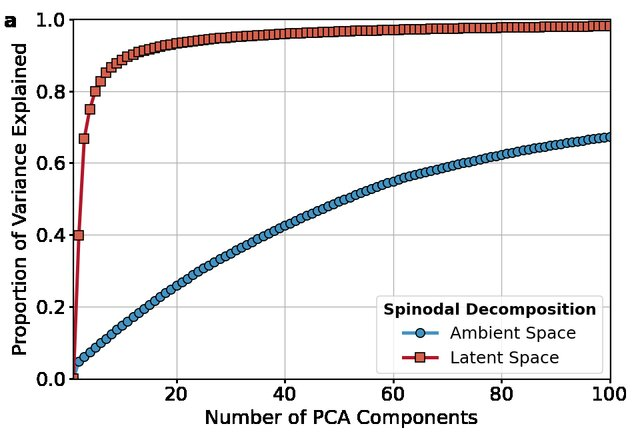
\includegraphics[width=0.95\linewidth]{img/Chapter2/Variance.jpg}
		\\
		{\scriptsize Ambient space (xanh) vs. Latent space (đỏ): thông tin được dồn nén vào rất ít thành phần chính.}
	\end{columns}
\end{frame}